
\documentclass[11pt]{article}
\usepackage[margin=1in]{geometry}
\usepackage{amsmath,amssymb}
\usepackage{graphicx}
\usepackage{booktabs}
\usepackage[colorlinks=true,linkcolor=blue,citecolor=blue,urlcolor=blue]{hyperref}

\title{Do universal machine-learned interatomic potentials find the ground state of isolated clusters?
A preregistered benchmark}
\author{Singularity}
\date{\today}

\begin{document}
\maketitle

\begin{abstract}
Universal machine-learned interatomic potentials (uMLIPs) trained on crystalline DFT data are increasingly used to
search the energy landscape of nanoclusters. Their reliability for isolated clusters, whose low-coordinated atoms are
absent from the training data, has not been measured systematically. We ask a simple question: given the low-energy
isomers of a cluster computed with DFT, does the uMLIP identify the same ground state?

We answer it with a preregistered benchmark on the Quantum Cluster Database (PBE, 55 elements, 3--55 atoms). The
protocol was fixed before any comparison. We developed on 27 elements and confirmed once on 28 held-out elements
(1\,458 element--size groups, 13\,102 isomers).
\begin{itemize}
\item MACE-MP-0 ranks the DFT ground state first in 33.3\% of the groups (95\% CI 28.5--38.0\%), against 12.2\%
expected by chance. MACE-OMAT-0 does so in 41.8\% of the groups.
\item Errors on relative isomer energies are 10--17~meV/atom, comparable to the spacing between competing isomers.
\item The ground state is among the five lowest-energy candidates of the model in 80\% (MACE-MP-0) and 87\%
(MACE-OMAT-0) of the groups. Re-checking a handful of candidates with DFT is therefore a cheap and effective
remedy.
\end{itemize}
A pilot on six independent public isomer datasets gives the same picture (34\% against 18\% by chance), including
a case where the reference uses the training functional.
\end{abstract}

\section{Introduction}
Global optimisation of cluster structures requires many energy evaluations. DFT is too expensive for exhaustive
searches beyond a few tens of atoms, so machine-learned potentials are used as surrogates, either alone or as priors
in Bayesian searches~\cite{BEACON}. Universal potentials such as MACE-MP-0~\cite{MACEMP0}, trained on the Materials
Project trajectories, promise to make this possible without system-specific training.

\textit{What is known.}
\begin{itemize}
\item Benchmarks of uMLIPs focus on bulk properties: formation energies, elastic constants, phonons and relaxation
behaviour~\cite{MatbenchDiscovery,PhononBench}.
\item For supported nanoparticles, a recent study compared several uMLIPs with a domain-specific potential for Cu on
alumina~\cite{SupportedNP}.
\item For isolated clusters the evidence is anecdotal. In the BEACON study of a 20-atom copper cluster, random
structure search with MACE-MP-0 alone did not locate the DFT global minimum in 1000 relaxations~\cite{BEACON}.
\end{itemize}

\textit{This work.} We measure, across many elements and sizes, how often a uMLIP ranks the DFT ground state first
among the low-energy isomers of a cluster, and how large its errors on relative isomer energies are. The protocol was
fixed before the reference data were inspected.

\section{Pilot study on public isomer datasets}
\label{sec:pilot}
We used six public datasets of low-lying cluster isomers with DFT energies
(Table~\ref{tab:pilot}). For each element--size group with at least two isomers, the energy of every isomer was
computed with the uMLIP at the DFT geometry (single point), and the isomer of lowest uMLIP energy was compared with
the DFT ground state.

\begin{table}[h]
\centering
\begin{tabular}{llccc}
\toprule
family & reference & ground state found & by chance & mean $|\Delta E_{\rm rel}|$ \\
\midrule
Ag$_n$, $n=3$--12 & B3PW91/def2-TZVP & 5/10 & 3.2/10 & --- \\
MoSn$_n$, $n=3$--16 & PBE/def2-TZVP & 4/15 & 1.3/15 & 0.22 eV \\
MgPt$_n$, $n=3$--12 & PBE0/def2-TZVP & 1/10 & 1.2/10 & 0.43 eV \\
PtSi$_n$, $n=2$--11 & PBE0/def2-TZVP & 3/10 & 1.6/10 & 0.30 eV \\
MB$_{12}$, 11 dopants & not stated & 6/11 & 2.7/11 & 1.08 eV \\
\midrule
total & & 19/56 (34\%) & 10.1/56 (18\%) & \\
\bottomrule
\end{tabular}
\caption{Pilot with MACE-MP-0 (medium). ``By chance'' is $\sum_g 1/m_g$, where $m_g$ is the number of isomers in
group $g$. The mean absolute error is over isomers within 1~eV of the DFT ground state.}
\label{tab:pilot}
\end{table}

\begin{figure}[h]
\centering
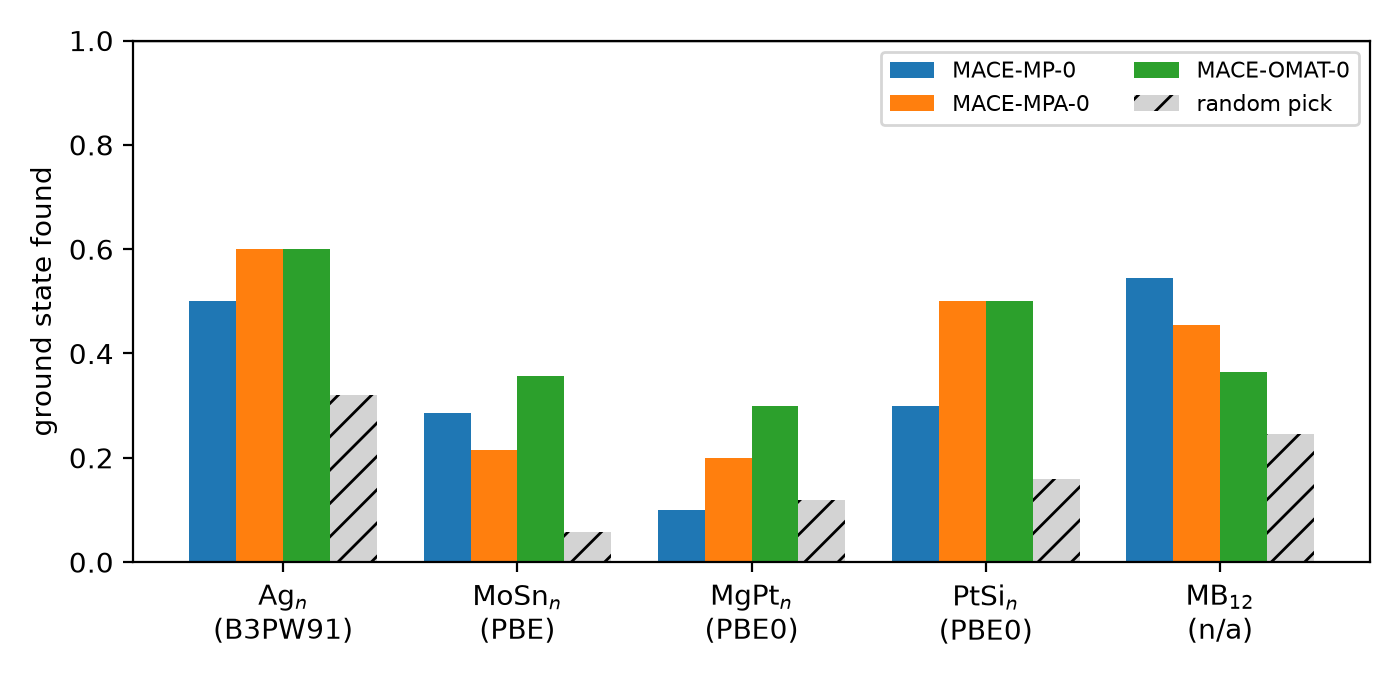
\includegraphics[width=0.85\textwidth]{fig_pilot.png}
\caption{Pilot: fraction of element--size groups (with at least three isomers) in which the uMLIP single-point
energies rank the DFT ground state first, for three MACE foundation models, compared with a random pick.}
\label{fig:pilot}
\end{figure}

\textit{Findings of the pilot.}
\begin{itemize}
\item The newer MACE-MPA-0 and MACE-OMAT-0 models change the picture little: over 55 groups with at least three isomers they find the ground state in 21 and 23 cases, against 19 for MACE-MP-0 and about 9.6 expected by chance.
\item Relaxing the DFT isomers with the uMLIP moves them by less than 0.2~\AA{} in most cases: the potentials
recognise the geometries but misorder them.
\item A linear correction in simple geometric descriptors (mean coordination, fraction of low-coordinated atoms,
dopant coordination), validated by leaving out one size at a time, does not improve the ranking on MoSn$_n$.
\end{itemize}
Only the MoSn$_n$ reference uses the training functional. Elsewhere the error mixes uMLIP limitations with
functional differences, which motivates the PBE benchmark below.

\section{Preregistered benchmark on the Quantum Cluster Database}
\label{sec:protocol}
\textit{Data.} The Quantum Cluster Database (QCD)~\cite{QCD} contains 61\,689 low-energy structures of clusters
of 55 elements with 3--55 atoms. Their energies were computed with spin-polarised PBE. Each element--size pair
forms a group of isomers, and the reference energy is the DFT energy at the stored geometry.

\textit{Selection.} We keep groups with at least three isomers whose DFT energies span at least 0.05~eV. To bound
the computing time, at most the ten lowest-energy isomers per group are retained; this cap was fixed before any
energy was compared with a model.

\textit{Split.} The 55 elements were shuffled with a fixed seed. Of the shuffled list, the first 27 elements
(1\,393 groups, 11\,790 isomers) were used for development and the remaining 28 (1\,458 groups, 13\,102 isomers)
for a single confirmation.

\textit{Models and metrics.} The primary model is MACE-MP-0 (medium) and the secondary model is MACE-OMAT-0
(medium). Both were run in double precision on CPU, as single points at the QCD geometries. The metrics were fixed
before the confirmation:
\begin{enumerate}
\item the fraction of groups in which the model's lowest-energy isomer is the DFT ground state (primary metric),
compared with the random-pick expectation $\langle 1/m_g\rangle$, where $m_g$ is the number of isomers in group
$g$;
\item the mean Spearman correlation between the model and DFT orderings;
\item the mean absolute error on relative energies of isomers within 0.5~eV of the ground state, in meV/atom;
\item all of the above by size class (3--10, 11--25 and 26--55 atoms).
\end{enumerate}

\textit{Hypotheses (preregistered).} H1: on the confirmation elements, MACE-MP-0 finds the ground state in fewer than
60\% of the groups. H2: MACE-OMAT-0 does not exceed MACE-MP-0 by more than 15 percentage points. H3: the error is
larger for small clusters (3--10 atoms) than for large ones (26--55 atoms).

The protocol was committed and tagged before the reference energies were compared with any model.

\section{Results}
\textit{Development.} On the 27 development elements, MACE-MP-0 found the ground state in 32.8\% of the groups
(random pick: 13.3\%). An exploratory test of whether the errors come from magnetism, which a spin-free potential
cannot represent, was negative: groups whose isomers all share the same magnetic moment were not easier
(25\% against 36\%).

\textit{Confirmation.} Table~\ref{tab:conf} and Fig.~\ref{fig:qcd} report the single confirmation run on the 28
held-out elements.
\begin{itemize}
\item \textbf{H1 is confirmed.} MACE-MP-0 finds the DFT ground state in 33.3\% of the groups, with a 95\%
confidence interval of 28.5--38.0\% from a bootstrap over elements. This is well below 60\% and well above the
12.2\% expected by chance.
\item \textbf{H2 is confirmed.} MACE-OMAT-0 is better by 8.4 percentage points (95\% CI 4.8--11.9), at 41.8\%. The
gain is real but well short of making the model reliable.
\item \textbf{H3 is only partly confirmed.} The error per atom is clearly larger for small clusters (39.5 against
8.3~meV/atom for MACE-MP-0). The ground-state hit rate, however, is not lower for 3--10 atoms than for 26--55
atoms; the intermediate class (11--25 atoms) is the worst.
\end{itemize}

\begin{table}[h]
\centering
\begin{tabular}{lccc}
\toprule
 & MACE-MP-0 & MACE-OMAT-0 & random pick \\
\midrule
ground state found (all) & \textbf{33.3\%} & \textbf{41.8\%} & 12.2\% \\
\quad 3--10 atoms & 36.3\% & 47.6\% & 12.2\% \\
\quad 11--25 atoms & 26.2\% & 33.4\% & 11.3\% \\
\quad 26--55 atoms & 36.1\% & 44.4\% & 12.7\% \\
mean Spearman $\rho$ & 0.31 & 0.47 & 0 \\
MAE, isomers within 0.5 eV (meV/atom) & 17.2 & 10.0 & --- \\
\bottomrule
\end{tabular}
\caption{Preregistered confirmation on 28 held-out elements of the QCD (1\,458 groups, 13\,102 isomers).}
\label{tab:conf}
\end{table}

\begin{figure}[h]
\centering
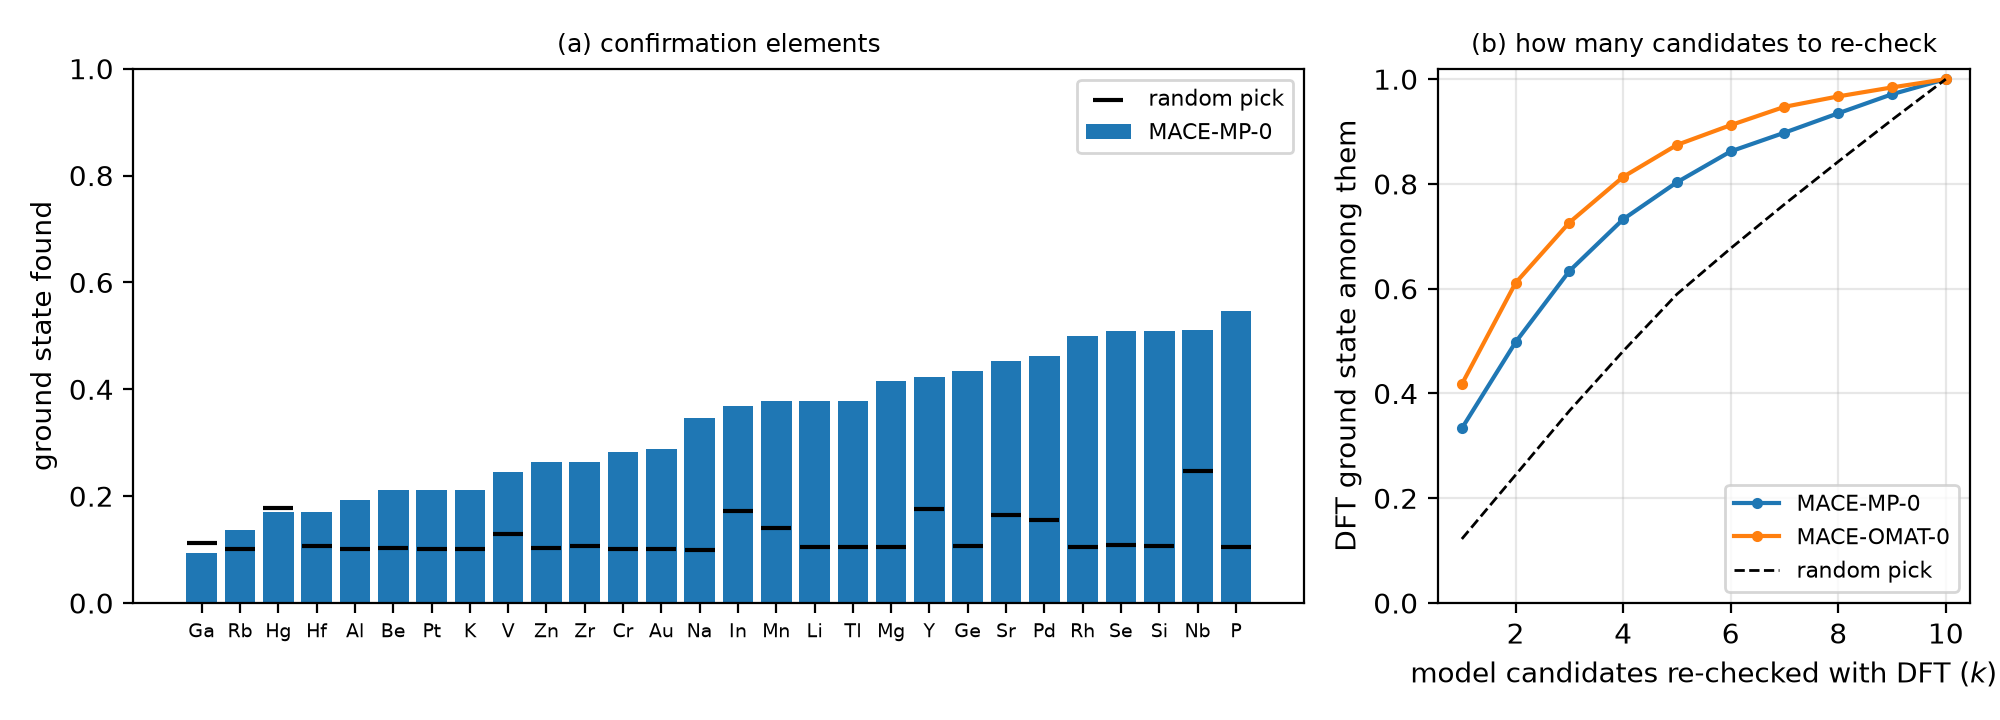
\includegraphics[width=\textwidth]{fig_qcd.png}
\caption{Confirmation set. (a) Fraction of groups in which MACE-MP-0 ranks the DFT ground state first, per element,
with the random-pick expectation (black ticks). (b) Fraction of groups in which the DFT ground state is among the $k$
lowest-energy candidates of the model (exploratory analysis).}
\label{fig:qcd}
\end{figure}

\textit{Exploratory: how many candidates to re-check.} If the $k$ lowest-energy isomers according to the model are
re-evaluated with DFT, the ground state is recovered in 33/50/63/80\% of the groups for $k=1/2/3/5$ with MACE-MP-0,
and in 42/61/73/87\% with MACE-OMAT-0 (Fig.~\ref{fig:qcd}b).
\begin{itemize}
\item The elements on which MACE-MP-0 is no better than chance include Ga, Rb and Hg.
\item Pt and Au, central to cluster catalysis, are found in only 21\% and 29\% of their groups.
\end{itemize}

\section{Discussion}
Universal potentials trained on crystals recognise cluster geometries: in the Ag$_n$ pilot, relaxing the DFT isomers with them moved the
atoms by less than 0.2~\AA{} in most cases. They do not, however, resolve the small energy differences between
competing isomers. The isomers lie within a few tens of meV/atom of each other, which is comparable to the model
errors, so the ranking is close to the noise level. This holds even when the reference functional (PBE) matches
the training data. In practice, three consequences follow.
\begin{enumerate}
\item \textbf{Do not trust the model's single lowest-energy structure.} In a cluster structure search, a uMLIP is a
good \emph{filter} but a poor \emph{judge}. Re-evaluating its five best candidates with DFT recovers the ground
state in 80--87\% of the cases at a modest cost.
\item \textbf{Conclusions drawn on uMLIP-only ground states need caution.} This applies to catalytic activity or
optical properties computed on a single uMLIP ground state, especially for Pt and Au clusters.
\item \textbf{Training data should include finite clusters.} The newer MACE-OMAT-0, trained on far more
off-equilibrium data, improves by only 8 points: more bulk data alone does not close the gap.
\end{enumerate}

\textit{Limitations.}
\begin{itemize}
\item The benchmark uses single points at DFT geometries and the low-energy isomers stored in the QCD. It measures
\emph{ranking}, not the full global search. A model could also find spurious minima that the QCD does not contain,
which would make the picture worse.
\item The QCD's own structures were partly found with machine-learned potentials before DFT refinement. Its ground
states could therefore be incomplete, but the reference energies are DFT.
\item Only two MACE models were tested in the confirmation.
\end{itemize}

\textit{Reproducibility.} The protocol, code, development and confirmation metrics are provided as ancillary files.
The QCD is available under CC-BY 4.0 from its authors.

\begin{thebibliography}{9}
\bibitem{MACEMP0} I. Batatia et al., ``A foundation model for atomistic materials chemistry,'' arXiv:2401.00096;
J. Chem. Phys. (2025).
\bibitem{BEACON} ``Bayesian optimization of atomic structures with prior probabilities from universal interatomic
potentials,'' arXiv:2408.15590.
\bibitem{SupportedNP} ``Benchmarking universal machine learning interatomic potentials for supported
nanoparticles,'' arXiv:2512.05221.
\bibitem{MatbenchDiscovery} J. Riebesell et al., ``Matbench Discovery,'' arXiv:2308.14920.
\bibitem{PhononBench} ``Universal machine learning interatomic potentials are ready for phonons,'' arXiv:2412.16551.
\bibitem{QCD} S. Manna et al., ``A database of low-energy atomically precise nanoclusters,'' Sci. Data 10, 308
(2023).
\end{thebibliography}

\end{document}
